\usepackage{ifthen}

% Define an agenda item
%
% Arguments:
% 1: Identifier of the agenda item, should be all lower-case
% 2: Type of the agenda item: lecture or lab
% 3: English title of the agenda item
% 4: English full description of the agenda item
% 5: French title of the agenda item
% 6: French full description of the agenda item
\newcommand\defagendaitem[6]{
  \ifthenelse{\equal{\agendalanguage}{french}}{
    \expandafter\def\csname #1@#2@title\endcsname {#5}
    \expandafter\def\csname #1@#2@contents\endcsname {#6}
  }{
    \expandafter\def\csname #1@#2@title\endcsname {#3}
    \expandafter\def\csname #1@#2@contents\endcsname {#4}
  }
}

% Show/render an agenda item
%
% Arguments:
% 1: Identifier of the agenda item, as defined by \defagendaitem
% 2: Type of the agenda item: lecture or lab
\newcommand\showagendaitem[2]{
  \ifthenelse{\boolean{hlineneeded}}{\\\hline}{\setboolean{hlineneeded}{true}}
    \ifthenelse{\equal{\agendalanguage}{french}}{
      \ifthenelse{\equal{#2}{lecture}}
      {Cours &}
      {
        \ifthenelse{\equal{#2}{lab}}{
          \ifthenelse{\equal{\trainingtype}{online}}{Démo &}{TP &}
        }
        {}
      }
    }{
      \ifthenelse{\equal{#2}{lecture}}
      {Lecture &}
      {
        \ifthenelse{\equal{#2}{lab}}{
          \ifthenelse{\equal{\trainingtype}{online}}{Demo &}{Lab &}
        }
        {}
      }
    }
    \csname #1@#2@title\endcsname &
    \vspace{-8pt}
    \csname #1@#2@contents\endcsname
}

% Define a board
%
% Arguments:
% 1: Identifier for the board, must be all lower-case
% 2: English title
% 3: English full description
% 4: French title
% 5: French full description
% 6: Board picture
\newcommand\defboard[6]{
  \ifthenelse{\equal{\agendalanguage}{french}}{
    \expandafter\def\csname #1@title\endcsname {#4}
    \expandafter\def\csname #1@contents\endcsname {#5}
  }{
    \expandafter\def\csname #1@title\endcsname {#2}
    \expandafter\def\csname #1@contents\endcsname {#3}
  }
  \expandafter\def\csname #1@image\endcsname {#6}
}

% Show/render a board
%
% Arguments:
% 1: Identifier of the board, as defined by \defboard
\newcommand\showboarditem[1]{
  \begin{tabularx}{\textwidth}{p{7cm}p{11cm}}
    \arrayrulecolor{blorange}
    \hline
    \multicolumn{1}{l}{\textbf{\textcolor{blorange}{\large \csname #1@title\endcsname}}} & \\
    \hline
    \arrayrulecolor{gray}
    \csname #1@contents\endcsname &
    \csname #1@image\endcsname \\
  \end{tabularx}
}

% Start an agenda by finding
% out if it is a morning or an
% afternoon if the training
% takes place on site
%
% Arguments:
% 1: Number of the half-day
\newcommand\showagendaday[1]{
  \arrayrulecolor{blorange}
  \\\hline
  \multicolumn{3}{l}{%
    \textbf{\textcolor{blorange}{\large\hspace{-1.5em}
      \ifthenelse{\equal{\trainingtype}{online}}{
        \showonlineagendaday{#1}
      }{
        \pgfmathparse{int(mod(#1, 2))}
        \ifnum\pgfmathresult=1
          \pgfmathparse{int((#1 + 1) / 2)}
          \showonsiteagendaday{\pgfmathresult}{morning}
        \else
          \pgfmathparse{int(#1 / 2)}
          \showonsiteagendaday{\pgfmathresult}{afternoon}
        \fi
      }
    }}
  } \\
  \hline
  \setboolean{hlineneeded}{false}
  \arrayrulecolor{gray}
}

% Start an online agenda half-day
%
% Arguments:
% 1: Number of the half-day
\newcommand\showonlineagendaday[1]{
  \ifthenelse{\equal{\agendalanguage}{french}}{
    Demi-journée #1
  }{
    Half day #1
  }
}

% Start an on-site agenda half-day
%
% Arguments:
% 1: Number of the day
% 2: "morning" or "afternoon"
\newcommand\showonsiteagendaday[2]{
  \ifthenelse{\equal{\agendalanguage}{french}}{
    \ifthenelse{\equal{#2}{morning}}{
      Jour #1 - Matin
    }{
      Jour #1 - Après-midi
    }
  }{
    \ifthenelse{\equal{#2}{morning}}{
      Day #1 - Morning
    }{
      Day #1 - Afternoon
    }
  }
}

\defboard
{stm32mp1}
{STM32MP1 Discovery Kit}
{
  One of these Discovery Kits from STMicroelectronics: {\bf
  STM32MP157A-DK1}, {\bf STM32MP157D-DK1}, {\bf STM32MP157C-DK2} or
  {\bf STM32MP157F-DK2}
  \begin{itemize}
  \item STM32MP157, dual Cortex-A7 processor from STMicroelectronics
  \item USB powered
  \item 512 MB DDR3L RAM
  \item Gigabit Ethernet port
  \item 4 USB 2.0 host ports
  \item 1 USB-C OTG port
  \item 1 Micro SD slot
  \item On-board ST-LINK/V2-1 debugger
  \item Arduino compatible headers
  \item Audio codec, buttons, LEDs
  \item LCD touchscreen (DK2 kits only)
  \vspace{-0.7cm}
  \end{itemize}
}
{Plateforme STM32MP1}
{
  Une de ces cartes de STMicroelectronics : {\bf
  STM32MP157A-DK1}, {\bf STM32MP157D-DK1}, {\bf STM32MP157C-DK2} ou
  {\bf STM32MP157F-DK2}
  \begin{itemize}
  \item Processeur STM32MP157, double Cortex-A7, de STMicroelectronics
  \item Alimentée par USB
  \item 512 Mo DDR3L RAM
  \item Port Gigabit Ethernet port
  \item 4 ports hôte USB 2.0
  \item 1 port USB-C OTG
  \item 1 connecteur Micro SD
  \item Debugger ST-LINK/V2-1 sur la carte
  \item Connecteurs compatibles Arduino Uno v3
  \item Codec audio
  \item Divers : boutons, LEDs
  \item Écran LCD tactile (uniquement sur cartes DK2)
  \vspace{-0.7cm}
  \end{itemize}
}
{
  \begin{center}
    \includegraphics[width=5cm]{../slides/discovery-board-dk1/discovery-board-dk1.png}
  \end{center}
}

\defagendaitem
{qna}
{misc}
{Questions and Answers}
{
  \begin{itemize}
  \item Questions and answers with the audience about the course topics
  \item Extra presentations if time is left, according what most
        participants are interested in.
  \end{itemize}
}
{Questions / réponses}
{
  \begin{itemize}
  \item Questions et réponses avec les participants à propos des sujets abordés.
  \item Présentations supplémentaires s'il reste du temps, en fonction des demandes
        de la majorité des participants.
  \end{itemize}
}


\defboard
{beagleboneblack}
{BeagleBone Black}
{
  {\bf BeagleBone Black} or {\bf BeagleBone Black Wireless} board
  \begin{itemize}
  \item An ARM AM335x (single Cortex-A8) processor from Texas
    Instruments
  \item USB powered
  \item 512 MB of RAM
  \item 2 or 4 GB of on-board eMMC storage
  \item USB host and device
  \item HDMI output
  \item 2 x 46 pins headers, to access UARTs, SPI buses, I2C buses
    and more.
  \item Ethernet or WiFi
  \end{itemize}
  \vspace{-0.7cm}
}
{BeagleBone Black}
{
  Carte {\bf BeagleBone Black} ou {\bf BeagleBone Black Wireless}
  \begin{itemize}
  \item Un processeur ARM AM335x de Texas Instruments (à base de
    Cortex-A8), avec accélération 3D, etc.
  \item 512 Mo de RAM
  \item 2 ou 4 Go de stockage eMMC
  \item USB hôte et device
  \item Sortie HDMI
  \item Connecteurs à 2 x 46 broches, pour accéder aux UARTs, aux bus
    SPI, aux bus I2C, et à d'autres entrées/sorties du processeur.
  \item Ethernet ou WiFi
  \vspace{-0.7cm}
  \end{itemize}
}
{
  \begin{center}
    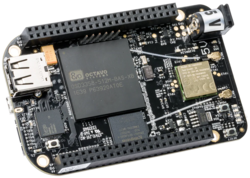
\includegraphics[width=5cm]{../slides/beagleboneblack-board/beagleboneblack_sd.png}
  \end{center}
}

\defboard
{beagleplay}
{BeaglePlay}
{
  {\bf BeaglePlay} board
  \begin{itemize}
    \item Texas Instruments AM625x (4xARM Cortex-A53 CPU)
    \item SoC with 3D acceleration, integrated MCU and many other peripherals.
    \item 2 GB of RAM
    \item 16 GB of on-board eMMC storage
    \item USB host and USB device, microSD, HDMI
    \item 2.4 and 5 GHz WiFi, Bluetooth and also Ethernet
    \item 1 MicroBus Header (SPI, I2C, UART, ...), OLDI and CSI connector.
  \vspace{-0.7cm}
  \end{itemize}
}
{BeaglePlay}
{
  Carte {\bf BeaglePlay}
  \begin{itemize}
    \item SoC Texas Instruments AM625x (CPU 4xARM Cortex-A53)
    \item SoC avec accélération 3D, MCU intégré et de nombreux autres périphériques.
    \item 2 GB de RAM
    \item 16 Go de stockage eMMC
    \item USB hôte et device, microSD, HDMI
    \item WiFi 2.4 and 5 GHz, Bluetooth et aussi Ethernet
    \item 1 Header MicroBus (SPI, I2C, UART, ...), connecteurs OLDI et CSI.
  \vspace{-0.7cm}
  \end{itemize}
}
{
  \begin{center}
    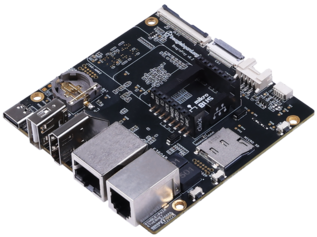
\includegraphics[width=5cm]{../slides/beagleplay-board/beagleplay_sd.png}
  \end{center}
}


\def \training{embedded-linux}

% Title
\ifthenelse{\equal{\agendalanguage}{french}}{
  \def \trainingtitle{Formation développement de systèmes Linux embarqué}
}{
  \def \trainingtitle{Embedded Linux system development training}
}

% Duration
\ifthenelse{\equal{\trainingtype}{online}}{
  \def \trainingduration{7}
}{
  \def \trainingduration{5}
}

\def \trainingicon{common/flaticon-embedded-linux-training.png}

% Training objectives
\ifthenelse{\equal{\agendalanguage}{french}}{
  \def \traininggoals{
    \begin{itemize}
    \item Être capable d'appréhender l'architecture générale d'un
      système Linux embarqué.
    \item Être capable de sélectionner, construire, mettre en oeuvre et
      utiliser une chaîne de compilation croisée.
    \item Être capable de comprendre la séquence d'un démarrage d'un
      système Linux embarqué et de mettre en oeuvre et d'utiliser le
      chargeur de démarrage U-Boot.
    \item Être capable de sélectionner une version du noyau Linux, de
      configurer, de compiler et d'installer le noyau Linux sur un
      système embarqué.
    \item Être capable de créer à partir de zéro un système de fichiers
      racine Linux, en comprenant les différents éléments qui le
      composent: répertoires, applications, bibliothèques, fichiers de
      configuration.
    \item Être capable de choisir et de mettre en oeuvre les principaux
      systèmes de fichiers Linux pour périphérique de stockage en mode
      bloc et flash, et de connaître leurs principales caractéristiques.
    \item Être capable d'interagir avec les périphériques matériels, de
      configurer le noyau avec les pilotes de périphériques nécessaires
      et d'étendre le {\em Device Tree}
    \item Être capable de sélectionner, de cross-compiler et d'intégrer
      des composants logiciels open-source (bibliothèques, applications)
      dans un système Linux embarqué, et de traiter la mise en
      conformité avec les licences open-source.
    \item Être capable de mettre en oeuvre un système de build Linux
      embarqué, pour construire un système complet pour une plateforme
      embarquée.
    \item Être capable de développer et débugger des applications sur un
      système Linux embarqué.
    \end{itemize}
  }
}{
  \def \traininggoals{
    \begin{itemize}
    \item Be able to understand the overall architecture of Embedded
      Linux systems.
    \item Be able to choose, build, setup and use a cross-compilation
      toolchain.
    \item Be able to understand the booting sequence of an embedded
      Linux system, and to set up and use the U-Boot bootloader.
    \item Be able to select a Linux kernel version, to configure, build
      and install the Linux kernel on an embedded system.
    \item Be able to create from scratch a Linux root filesystem,
      including all its elements: directories, applications,
      configuration files, libraries.
    \item Be able to choose and setup the main Linux filesystems for
      block and flash storage devices, and understand their main
      characteristics.
    \item Be able to interact with hardware devices, configure the
      kernel with appropriate drivers and extend the {\em Device Tree}
    \item Be able to select, cross-compile and integrate open-source
      software components (libraries, applications) in an Embedded Linux
      system, and to handle license compliance.
    \item Be able to setup and use an embedded Linux build system, to
      build a complete system for an embedded platform.
    \item Be able to develop and debug applications on an embedded Linux
      system.
    \end{itemize}
  }
}

% Training prerequisites
\def \trainingprerequisites{
  \begin{itemize}
    \prerequisitecommandline
    \prerequisiteenglish
  \end{itemize}
}

% Training audience
\ifthenelse{\equal{\agendalanguage}{french}}{
  \def \trainingaudience{
    Ingénieurs développant des systèmes embarqués
    reposant sur Linux et des composants open-source.
  }
}{
  \def \trainingaudience{
    People developing devices using the Linux kernel
    \newline People supporting embedded Linux system developers.
  }
}

\def \trainers {alexandre-belloni,alexis-lothore,antonin-godard,bastien-curutchet,gregory-clement,jeremie-dautheribes,joaomarcos-costa,luca-ceresoli,maxime-chevallier,mathieu-dubois-briand,miquel-raynal,richard-genoud,romain-gantois,thomas-petazzoni}

% Time ratio
\def \onsitelecturetimeratio{50}
\def \onsitelabtimeratio{50}

% Agenda items


\defagendaitem
{intro}
{lecture}
{Introduction to embedded Linux}
{
  \begin{itemize}
  \item Advantages of Linux versus traditional embedded operating
    systems.
  \item Typical hardware platforms used to run embedded Linux systems.
  \item Overall architecture of embedded Linux systems: overview of
    the major software components.
  \item Development environment for Embedded Linux development.
  \end{itemize}
}
{Introduction à Linux embarqué}
{
  \begin{itemize}
  \item Introduction au Logiciel Libre
  \item Atouts du Logiciel Libre pour les systèmes embarqués
  \item Exemples de systèmes embarqués fonctionnant sous Linux
  \item Besoins en CPU, RAM et stockage
  \item Choix d'une plateforme matérielle
  \item Architecture du système : composants principaux
  \item Différentes tâches pour développer un système embarqué
  \end{itemize}
}
\defagendaitem
{crosscompile}
{lecture}
{Cross-compiling toolchain and C library}
{
  \begin{itemize}
  \item What's inside a cross-compiling toolchain
  \item Choosing the target C library
  \item What's inside the C library
  \item Ready to use cross-compiling toolchains
  \item Building a cross-compiling toolchain with automated tools.
  \end{itemize}
}
{Chaîne de compilation croisée et bibliothèque standard C}
{
  \begin{itemize}
  \item Les composants d'une chaîne de compilation croisée.
  \item Choisir une bibliothèque standard C.
  \item Le contenu de la bibliothèque standard C.
  \item Les chaînes de compilation croisée prêtes à l'emploi.
  \item La construction automatisée d'une chaîne de compilation croisée.
  \end{itemize}
}
\defagendaitem
{crosscompile}
{lab}
{Cross compiling toolchain}
{
  \begin{itemize}
  \item Getting and configuring Crosstool-NG
  \item Executing it to build a custom cross-compilation toolchain
  \item Exploring the contents of the toolchain
  \end{itemize}
}
{Chaîne de compilation croisée}
{
  \begin{itemize}
  \item Configuration de Crosstool-NG
  \item Exécution pour construire une chaîne de compilation croisée
    personnalisée reposant sur la uClibc.
  \item Exploration du contenu d'une chaîne de compilation croisée
  \end{itemize}
}
\defagendaitem
{bootprocess}
{lecture}
{Boot process, firmware, bootloaders}
{
  \begin{itemize}
  \item Booting process of embedded platforms, focus on the {\em x86}
    and {\em ARM} architectures
  \item Boot process and bootloaders on {\em x86} platforms (legacy
    and UEFI)
  \item Boot process on ARM platforms: ROM code, bootloaders, {\em ARM
      Trusted Firmware}
  \item Focus on U-Boot: configuration, installation, and usage.
  \item U-Boot commands, U-Boot environment, U-Boot scripts, U-Boot
    generic distro boot mechanism
  \end{itemize}
}
{Processus de démarrage, firmware, chargeurs de démarrage}
{
  \begin{itemize}
  \item Processus de démarrage des systèmes embarqués, focus sur les
    architectures {\em x86} et {\em ARM}
  \item Processus de démarrage et chargeurs de démarrage sur
    plateformes {\em x86} (legacy et UEFI)
  \item Processus de démarrage sur plateformes {\em ARM} : code en ROM,
    chargeurs de démarrage, {\em ARM Trusted Firmware}
  \item Focus sur U-Boot : configuration, installation et utilisation
  \item Commandes U-Boot, environnement U-Boot, scripts U-Boot,
    mécanisme {\em distro boot command} de U-Boot
  \end{itemize}
}
\defagendaitem
{uboot}
{lab}
{Bootloader and U-boot}
{
  \begin{itemize}
  \item Set up serial communication with the board.
  \item Configure, compile and install U-Boot for the target hardware.
  \item Only on STM32MP1: configure, compile and install Trusted Firmware-A
  \item Become familiar with U-Boot environment and commands.
  \item Set up TFTP communication with the board. Use TFTP U-Boot
    commands.
  \end{itemize}
}
{U-Boot}
{
  \begin{itemize}
  \item Mise en place de la communication série avec la carte.
  \item Configuration, compilation et installation d'U-Boot sur la
    plateforme embarquée.
  \item Seulement sur STM32MP1 : Configuration, compilation et
    installation de Trusted Firmware-A sur la plateforme embarquée.
  \item Familiarisation avec l'environnement et les commandes
    d'U-Boot.
  \item Mise en place de la communication TFTP avec la carte.
    Utilisation des commandes TFTP d'U-Boot.
  \end{itemize}
}
\defagendaitem
{kernel}
{lecture}
{Linux kernel}
{
  \begin{itemize}
  \item Role and general architecture of the Linux kernel
  \item Separation between kernel and user-space, and interfaces
    between user-space and the Linux kernel
  \item Understanding Linux kernel versions: choosing between
    vendor-provided kernel and upstream kernel, {\em Long Term
      Support} versions
  \item Getting the Linux kernel source code
  \end{itemize}
}
{Noyau Linux}
{
  \begin{itemize}
  \item Rôle et architecture générale du noyau Linux.
  \item Séparation entre noyau et espace utilisateur, interfaces entre
    l'espace utilisateur et le noyau
  \item Comprendre les différentes versions du noyau Linux : choix
    entre versions proposées par les fabricants et la version {\em
      upstream}, versions {\em Long Term Support}
  \item Récupérer les sources du noyau Linux
  \end{itemize}
}
\defagendaitem
{fetchkernel}
{lab}
{Fetching Linux kernel sources}
{
  \begin{itemize}
  \item Clone the mainline Linux tree
  \item Accessing stable releases
  \end{itemize}
}
{Récupération des sources du noyau Linux}
{
  \begin{itemize}
  \item Clonage du dépôt git officiel de Linux
  \item Accès aux versions stables
  \end{itemize}
}
\defagendaitem
{configurekernel}
{lecture}
{Configuring, compiling and booting the Linux kernel}
{
  \begin{itemize}
  \item Configuring the Linux kernel: ready-made configuration files,
    configuration interfaces
  \item Concept of {\em Device Tree}
  \item Cross-compiling the Linux kernel
  \item Study of the generated files and their role
  \item Installing and booting the Linux kernel
  \item The Linux kernel command line
  \end{itemize}
}
{Configuration, compilation et démarrage du Noyau Linux}
{
  \begin{itemize}
  \item Configuration du noyau Linux : configuration pré-définies,
    interfaces de configuration
  \item Concept de {\em Device Tree}
  \item Cross-compilation du noyau Linux
  \item Rôle des fichiers résultants de la compilation du noyau Linux
  \item Installation et démarrage du noyau Linux
  \item La ligne de commande du noyau Linux
  \end{itemize}
}
\defagendaitem
{compilekernel}
{lab}
{Kernel cross-compiling and booting}
{
  \begin{itemize}
  \item Configuring the Linux kernel and cross-compiling it for the
    embedded hardware platform.
  \item Downloading your kernel on the board through U-boot's TFTP
    client.
  \item Booting your kernel.
  \item Automating the kernel boot process with U-Boot scripts.
  \end{itemize}
}
{Compilation croisée du noyau et démarrage sur la carte}
{
  \begin{itemize}
  \item Configuration du noyau Linux et compilation croisée pour la
    plateforme embarquée.
  \item Téléchargement du noyau en utilisant le client TFTP d'U-Boot.
  \item Démarrage du noyau depuis la RAM.
  \item Automatisation du démarrage du noyau avec des scripts U-Boot.
  \end{itemize}
}
\defagendaitem
{rootfs}
{lecture}
{Root filesystem in Linux}
{
  \begin{itemize}
  \item Filesystems in Linux.
  \item Role and organization of the root filesystem.
  \item Location of the root filesystem: on storage, in memory,
        from the network.
  \item Device files, virtual filesystems.
  \item Contents of a typical root filesystem.
  \end{itemize}
}
{Système de fichier racine}
{
  \begin{itemize}
  \item Les systèmes de fichiers dans Linux.
  \item Rôle et organisation du système de fichiers racine.
  \item Localisation de ce système de fichiers : sur espace
	de stockage, en mémoire, sur le réseau.
  \item Les fichiers device, les systèmes de fichiers virtuels.
  \item Contenu type d'un système de fichiers racine.
  \end{itemize}
}
\defagendaitem
{busybox}
{lecture}
{BusyBox}
{
  \begin{itemize}
  \item Detailed overview. Detailed features.
  \item Configuration, compiling and deploying.
  \end{itemize}
}
{BusyBox}
{
  \begin{itemize}
  \item Présentation de BusyBox. Intérêt pour les systèmes embarqués.
  \item Configuration, compilation et installation.
  \end{itemize}
}
\defagendaitem
{busybox}
{lab}
{Tiny root filesystem built from scratch with BusyBox}
{
  \begin{itemize}
  \item Setting up a kernel to boot your system on a workstation
    directory exported by NFS
  \item Passing kernel command line parameters to boot on NFS
  \item Creating the full root filesystem from scratch.
    Populating it with BusyBox based utilities.
  \item System startup using BusyBox \code{init}
  \item Using the BusyBox HTTP server.
  \item Controlling the target from a web browser on the PC host.
  \item Setting up shared libraries on the target and compiling
    a sample executable.
  \end{itemize}
}
{Construction d'un minuscule système Linux embarqué avec BusyBox}
{
  \begin{itemize}
  \item Construction à partir de zéro d'un système de fichiers racine
    contenant un système Linux embarqué
  \item Mise en place d'un noyau permettant de démarrer le système
    depuis un répertoire mis à disposition par la station de
    développement au travers de NFS.
  \item Passage de paramètres au noyau pour le démarrage avec NFS.
  \item Création complète du système de fichiers à partir de zéro :
    installation de BusyBox, création des fichiers spéciaux pour les
    périphériques.
  \item Initialisation du système en utilisant le programme init de BusyBox.
  \item Utilisation du serveur HTTP de BusyBox.
  \item Contrôle de la cible à partir d'un navigateur Web sur la
    station de développement.
  \item Mise en place des bibliothèques partagées sur la cible et
    développement d'une application d'exemple.
  \end{itemize}
}
\defagendaitem
{accessinghardware}
{lecture}
{Accessing hardware devices}
{
  \begin{itemize}
  \item How to access hardware on popular busses: USB, SPI, I2C, PCI
  \item Usage of kernel drivers and direct user-space access
  \item The {\em Device Tree} syntax, and how to use it to describe
    additional devices and pin-muxing
  \item Finding Linux kernel drivers for specific hardware devices
  \item Using kernel modules
  \item Hardware access using \code{/dev} and \code{/sys}
  \item User-space interfaces for the most common hardware devices:
    storage, network, GPIO, LEDs, audio, graphics, video
  \end{itemize}
}
{Accès aux périphériques matériels}
{
  \begin{itemize}
  \item Comment accéder au matériel sur les principaux bus : USB, SPI,
    I2C, PCI
  \item Utilisation de pilotes de périphériques dans le noyau ou accès
    depuis l'espace utilisateur
  \item La syntaxe du {\em Device Tree}, et comment l'utilisation pour
    décrire des périphériques additionnels et le multiplexage des
    signaux.
  \item Trouver des pilotes de périphériques dans le noyau Linux pour
    des périphériques matériels.
  \item Utilisation de modules noyau
  \item Accès au matériel par \code{/dev} ou \code{/sys}
  \item Interfaces en espace utilisateur pour les périphériques les
    plus courants : stockage, réseau, GPIO, LEDs, audio, affichage,
    video
  \end{itemize}
}
\defagendaitem
{accessinghardware}
{lab}
{Accessing hardware devices}
{
  \begin{itemize}
  \item Exploring the contents of \code{/dev} and \code{/sys} and the
    devices available on the embedded hardware platform.
  \item Using GPIOs and LEDs.
  \item Modifying the Device Tree to control pin multiplexing and
        to declare an I2C-connected joystick.
  \item Adding support for a USB audio card using Linux kernel modules
  \item Adding support for the I2C-connected joystick through
        an out-of-tree module.
  \end{itemize}
}
{Accès aux périphériques matériels}
{
  \begin{itemize}
  \item Exploration du contenu de \code{/dev} et \code{/sys}, et des
    périphériques disponibles sur la plateforme embarquée.
  \item Utilisation de GPIOs et de LEDs.
  \item Modification du Device Tree pour controler le multiplexage
    de broches et déclarer un joystick connecté sur I2C.
  \item Ajout du support pour une carte son USB en utilisant des
    modules noyau.
  \item Prise en charge du joystick I2C par la compilation et
    l'installation d'un module noyau externe.
  \end{itemize}
}
\defagendaitem
{blockfs}
{lecture}
{Block filesystems}
{
  \begin{itemize}
  \item Accessing and partitioning block devices.
  \item Filesystems for block devices.
  \item Usefulness of journaled filesystems.
  \item Read-only block filesystems.
  \item RAM filesystems.
  \item How to create each of these filesystems.
  \item Suggestions for embedded systems.
  \end{itemize}
}
{Système de fichiers bloc}
{
  \begin{itemize}
  \item Accéder et partitionner des périphériques bloc.
  \item Systèmes de fichiers pour périphériques bloc.
  \item Utilité des systèmes de fichiers journalisés.
  \item Systèmes de fichiers en lecture seule.
  \item Systèmes de fichiers en RAM.
  \item Création de chacun de ces systèmes de fichiers.
  \item Suggestions pour les systèmes embarqués.
  \end{itemize}
}
\defagendaitem
{blockfs}
{lab}
{Block filesystems}
{
  \begin{itemize}
  \item Creating partitions on your SD card
  \item Booting a system with a mix of filesystems: {\em SquashFS} for
    the root filesystem, {\em ext4} for system data, and {\em
      tmpfs} for temporary system files.
  \end{itemize}
}
{Système de fichiers bloc}
{
  \begin{itemize}
  \item Créer des partitions sur le stockage bloc.
  \item Démarrage d'un système avec un assemblage de plusieurs systèmes
    de fichiers : SquashFS pour le système de fichier racine, ext4 pour
    les données du système et tmpfs pour les fichiers temporaires.
  \end{itemize}
}
\defagendaitem
{flashfs}
{lecture}
{Flash filesystems}
{
  \begin{itemize}
  \item The Memory Technology Devices (MTD) filesystem.
  \item Filesystems for MTD storage: JFFS2, Yaffs2, UBIFS.
  \item Kernel configuration options
  \item MTD storage partitions.
  \item Focus on today's best solution, UBI and UBIFS:
	preparing, flashing and using UBI images.
  \end{itemize}

  \vspace{0.5cm}

  {\em Note: as the embedded hardware platform used for the labs does
    not have any flash-based storage, this lecture will not be
    illustrated with a corresponding practical lab.}
}
{Système de fichiers pour flash}
{
  \begin{itemize}
  \item Le sous-système Memory Technology Devices du noyau Linux.
  \item Les systèmes de fichiers pour le stockage MTD : JFFS2, YAFFS2,
    UBIFS.
  \item Options de configuration du noyau.
  \item Partitions MTD.
  \item Étude en détail de UBI et UBIFS : préparation, flashage et mise
    en oeuvre d'images UBI.
  \end{itemize}

  \vspace{0.5cm}

  {\em Note : la plateforme embarquée utilisée pour les labs ne
    comportant pas de mémoire flash NAND en accès direct, cette partie
    du cours ne sera pas illustrée avec un TP correspondant.}
}
\defagendaitem
{crosscompileapp}
{lecture}
{Cross-compiling user-space libraries and applications}
{
  \begin{itemize}
  \item Configuring, cross-compiling and installing applications and
    libraries.
  \item Concept of build system, and overview of a few common build
    systems used by open-source projects: Makefile, {\em autotools},
    {\em CMake}, {\em meson}
  \item Overview of the common issues encountered when
    cross-compiling.
  \end{itemize}
}
{Cross-compilation de bibliothèques et d'applications espace utilisateur}
{
  \begin{itemize}
  \item Configuration, compilation croisée et installation
    d'applications et de bibliothèques
  \item Concept de {\em build system}, et aperçu de quelques {\em
      build systems} courants utilisés dans les projets open-source :
    {\em Makefile}, {\em autotools}, {\em CMake}, {\em meson}
  \item Aperçu des problématiques courantes rencontrées lors de la
    compilation croisée
  \end{itemize}
}
\defagendaitem
{crosscompileapp}
{lab}
{Cross-compiling applications and libraries}
{
  \begin{itemize}
  \item Manual cross-compilation of several open-source libraries and
    applications for an embedded platform.
  \item Learning about common pitfalls and issues, and their
    solutions.
  \item This includes compiling {\em alsa-utils} package,
    and using its \code{speaker-test} program to test that
    audio works on the target.
  \end{itemize}
}
{Compilation croisée de bibliothèques et d'applications}
{
  \begin{itemize}
  \item Compilation croisée manuelle de plusieurs bibliothèques et
    applications open-source pour une plateforme embarquée.
  \item Apprentissage des principales techniques et des problèmes
    principaux.
  \item Cela inclut la compilation du composant {\em alsa-utils},
     et l'utilisation de son programme \code{speaker-test} pour
     vérifier que l'audio fonctionne sur la cible.
  \end{itemize}
}
\defagendaitem
{buildsystem}
{lecture}
{Embedded system building tools}
{
  \begin{itemize}
  \item Approaches for building embedded Linux systems: build systems
    and binary distributions
  \item Principle of {\em build systems}, overview of Yocto
    Project/OpenEmbedded and Buildroot.
  \item Principle of {\em binary distributions} and useful tools,
    focus on Debian/Ubuntu
  \item Specialized software frameworks/distributions: Tizen, AGL,
    Android
  \end{itemize}
}
{Outils de construction de systèmes}
{
  \begin{itemize}
  \item Les différentes approches pour construire un système Linux
    embarqué : {\em build systems} et distributions binaires
  \item Principe d'un {\em build system}, aperçu de Yocto
    Project/OpenEmbedded et de Buildroot
  \item Principe d'une {\em distribution binaire} et outils associés,
    focus sur Debian et Ubuntu
  \item Piles logicielles standards : Tizen, AGL, Android
  \end{itemize}
}
\defagendaitem
{buildroot}
{lab}
{System build with Buildroot}
{
  \begin{itemize}
  \item Using Buildroot to rebuild the same basic system
        plus a sound playing server ({\em MPD}) and a
        client to control it ({\em mpc}).
  \item Driving music playback, directly from the target,
        and then remotely through an MPD client on the
	host machine.
  \item Analyzing dependencies between packages.
  \end{itemize}
}
{Construction d'un système avec Buildroot}
{
  \begin{itemize}
  \item Utilisation de Buildroot pour construire de façon automatisée
    le même système de base que dans le TP précédent, en y rajoutant
    un serveur pour jouer des bandes sonores ({\em MPD}) ainsi
    qu'un client pour piloter ce serveur ({\em mpc}).
  \item Contrôle de la lecture audio, directement depuis la
    cible, puis depuis un client MPD sur le PC de développement.
  \item Analyse des dépendences entre les différents composants
    du système.
  \end{itemize}
}
\defagendaitem
{license}
{lecture}
{Open source licenses and compliance}
{
  \begin{itemize}
  \item Presentation of the most important open-source licenses: GPL,
    LGPL, MIT, BSD, Apache, etc.
  \item Concept of {\em copyleft} licenses
  \item Differences between (L)GPL version 2 and 3
  \item Compliance with open-source licenses: best practices
  \end{itemize}
}
{Licences open-source et mise en conformité}
{
  \begin{itemize}
  \item Présentation des principales licenses open-source : GPL, LGPL,
    MIT, BSD, Apache, etc.
  \item Concept de {\em copyleft} dans les licences open-source
  \item Différence entre (L)GPL version 2 et 3
  \item Mise en conformité avec les licences open-source : bonnes
    pratiques
  \end{itemize}
}
\defagendaitem
{opensourcelinuxsoftwarestacks}
{lecture}
{Overview of major embedded Linux software stacks}
{
  \begin{itemize}
  \item \code{systemd} as an {\em init} system
  \item Hardware management with {\em udev}
  \item Inter-process communication with {\em D-Bus}
  \item The graphics software stack: DRM/KMS, X.org, Wayland, Qt, Gtk,
    OpenGL
  \item The multimedia software stack: Video4Linux, GStreamer,
    Pulseaudio, Pipewire
  \end{itemize}
}
{Aperçu des stack logicielles open-source majeures pour Linux embarqué}
{
  \begin{itemize}
  \item \code{systemd} comme système {\em init}
  \item Gestion du matériel avec {\em udev}
  \item Communication inter-processus avec {\em D-Bus}
  \item La stack logicielle pour le graphique : DRM/KMS, X.org,
    Wayland, Qt, Gtk, OpenGL
  \item La stack logicielle pour le multimédia : Video4Linux,
    GStreamer, Pulseaudio, Pipewire
  \end{itemize}
}
\defagendaitem
{integration}
{lab}
{Integration of additional software stacks}
{
  \begin{itemize}
  \item Integration of {\em systemd} as an init system
  \item Use {\em udev} built in {\em systemd} for automatic module
    loading
  \end{itemize}
}
{Intégration de stack logicielles additionnelles}
{
  \begin{itemize}
  \item Intégration de {\em systemd} comme système d'init
  \item Utilisation de {\em udev} pour le chargement automatique de
    modules
  \end{itemize}
}
\defagendaitem
{debugging}
{lecture}
{Application development and debugging}
{
  \begin{itemize}
  \item Programming languages and libraries available.
  \item Build system for your application, an overview of {\em CMake}
    and {\em meson}
  \item The {\em gdb} debugger: remote debugging with {\em gdbserver},
    post-mortem debugging with \code{core} files
  \item Performance analysis, tracing and profiling tools, memory
    checkers: \code{strace}, \code{ltrace}, \code{perf},
    \code{valgrind}
  \end{itemize}
}
{Développement et déboguage d'application}
{
  \begin{itemize}
  \item Langages de programmations et bibliothèques disponibles.
  \item {\em Build system} pour votre application, un aperçu de {\em
      CMake} et {\em Meson}
  \item Le débogueur {\em gdb} : déboguage d'applications à distance
    avec gdb et gdbserver, analyse post-mortem d'une application.
  \item Analyse de performance, outils de {\em tracing} et {\em
      profiling}, analyseurs mémoire : \code{strace}, \code{ltrace},
    \code{perf}, \code{valgrind}
  \end{itemize}
}
\defagendaitem
{debugging}
{lab}
{Application development and debugging}
{
  \begin{itemize}
  \item Creating an application that uses an I2C-connected joystick to
    control an audio player.
  \item Setting up an IDE to develop and remotely debug an
    application.
  \item Using {\em strace}, {\em ltrace}, {\em gdbserver} and {\em
      perf} to debug/investigate buggy applications on the embedded
    board.
  \end{itemize}
}
{Développement et déboguage d'application}
{
  \begin{itemize}
  \item Création d'une application qui utilise un joystick connecté
    sur I2C pour contrôler un player audio.
  \item Mise en place d'un IDE pour le développement et le déboguage
    d'une application.
  \item Utilisation de {\em strace}, {\em ltrace}, {\em gdbserver} et
    {\em perf} pour déboguer/investiguer des applications
    problématiques sur la plateforme embarquée.
  \end{itemize}
}
\defagendaitem
{resources}
{lecture}
{Useful resources}
{
  \begin{itemize}
  \item Books about embedded Linux and system programming
  \item Useful online resources
  \item International conferences
  \end{itemize}
}
{Ressources utiles}
{
  \begin{itemize}
  \item Livres sur Linux embarqué et la programmation système
  \item Ressources sur Internet
  \item Conférences internationales
  \end{itemize}
}

\def \agendaboards{stm32mp1,beagleboneblack,beagleplay}

\def \onlineagenda {
  \ifthenelse{\equal{\agendalanguage}{french}}{
    \section{Programme de la formation}
  }{
    \section{Training Schedule}
  }
  \begin{tabularx}{\textwidth}{p{2cm}p{5cm}p{11cm}}
  \showagendaday{1}
  \showagendaitem{intro}{lecture}
  \showagendaitem{crosscompile}{lecture}
  \showagendaitem{crosscompile}{lab}
  \showagendaitem{bootprocess}{lecture}
  \showagendaday{2}
  \showagendaitem{uboot}{lab}
  \showagendaitem{kernel}{lecture}
  \showagendaitem{fetchkernel}{lab}
  \showagendaitem{configurekernel}{lecture}
  \showagendaitem{compilekernel}{lab}
  \showagendaday{3}
  \showagendaitem{rootfs}{lecture}
  \showagendaitem{busybox}{lecture}
  \showagendaitem{busybox}{lab}
  \showagendaday{4}
  \showagendaitem{accessinghardware}{lecture}
  \showagendaitem{accessinghardware}{lab}
  \showagendaitem{blockfs}{lecture}
  \showagendaitem{blockfs}{lab}
  \showagendaday{5}
  \showagendaitem{flashfs}{lecture}
  \showagendaitem{crosscompileapp}{lecture}
  \showagendaitem{crosscompileapp}{lab}
  \showagendaday{6}
  \showagendaitem{buildsystem}{lecture}
  \showagendaitem{buildroot}{lab}
  \showagendaitem{license}{lecture}
  \showagendaitem{opensourcelinuxsoftwarestacks}{lecture}
  \showagendaday{7}
  \showagendaitem{integration}{lab}
  \showagendaitem{debugging}{lecture}
  \showagendaitem{debugging}{lab}
  \showagendaitem{resources}{lecture}
  \end{tabularx}
}

\def \onsiteagenda {
  \ifthenelse{\equal{\agendalanguage}{french}}{
    \section{Programme de la formation}
  }{
    \section{Training Schedule}
  }
  \begin{tabularx}{\textwidth}{p{2cm}p{5cm}p{11cm}}
  \showagendaday{1}
  \showagendaitem{intro}{lecture}
  \showagendaitem{crosscompile}{lecture}
  \showagendaitem{crosscompile}{lab}
  \showagendaday{2}
  \showagendaitem{bootprocess}{lecture}
  \showagendaitem{uboot}{lab}
  \showagendaday{3}
  \showagendaitem{kernel}{lecture}
  \showagendaitem{fetchkernel}{lab}
  \showagendaitem{configurekernel}{lecture}
  \showagendaitem{compilekernel}{lab}
  \showagendaday{4}
  \showagendaitem{rootfs}{lecture}
  \showagendaitem{busybox}{lecture}
  \showagendaitem{busybox}{lab}
  \showagendaday{5}
  \showagendaitem{accessinghardware}{lecture}
  \showagendaitem{accessinghardware}{lab}
  \showagendaday{6}
  \showagendaitem{blockfs}{lecture}
  \showagendaitem{blockfs}{lab}
  \showagendaitem{flashfs}{lecture}
  \showagendaday{7}
  \showagendaitem{crosscompileapp}{lecture}
  \showagendaitem{crosscompileapp}{lab}
  \showagendaday{8}
  \showagendaitem{buildsystem}{lecture}
  \showagendaitem{buildroot}{lab}
  \showagendaitem{license}{lecture}
  \showagendaday{9}
  \showagendaitem{opensourcelinuxsoftwarestacks}{lecture}
  \showagendaitem{integration}{lab}
  \showagendaday{10}
  \showagendaitem{debugging}{lecture}
  \showagendaitem{debugging}{lab}
  \showagendaitem{resources}{lecture}
  \end{tabularx}
}
